\documentclass[a4paper,oneside,12pt]{extarticle}

\usepackage[utf8]{inputenc}
\usepackage[english]{babel}
\usepackage{amssymb,amsthm,mathtools,enumitem,geometry,hyperref,booktabs}
\usepackage{graphicx}
\usepackage{xcolor}
\usepackage{tikz}
\usetikzlibrary{calc,patterns,decorations.pathreplacing}
\usepackage{tikz-cd}
\usepackage{pgfplots}
\usepgfplotslibrary{fillbetween}
\pgfplotsset{compat=1.18}
\usepackage{float}

\geometry{lmargin=15mm,rmargin=15mm,tmargin=10mm,bmargin=10mm,includeheadfoot}
\pagestyle{plain}
\frenchspacing

\theoremstyle{plain}
\newtheorem{proposition}{Proposition}
\newtheorem{lemma}[proposition]{Lemma}

\theoremstyle{definition}
\newtheorem{definition}[proposition]{Definition}
\newtheorem{example}[proposition]{Example}

\theoremstyle{remark}
\newtheorem{remark}[proposition]{Remark}

\newcommand*{\E}{\mathbb{E}}
\newcommand*{\Var}{\mathrm{Var}}
\newcommand*{\mP}{\mathbb{P}}
\newcommand*{\mR}{\mathbb{R}}
\newcommand*{\mbF}{\mathcal{F}}
\newcommand*{\ve}{\varepsilon}




\begin{document}
\begin{titlepage}
\begin{center}

{\footnotesize\scshape\color{gray}
Working Notes in Quantitative Risk and Modeling
}

\vfill

{\LARGE\bfseries Homoscedasticity and Its Testing:\\[4pt]
From Conditional Expectation to the Breusch--Pagan Test}

\vspace{36pt}

{\normalsize Boris Garbuzov}

\vfill

{\Large\bfseries Part~5~/~12}

\vspace{6pt}

{\Large\bfseries Worked Example: The Uniform Distribution\\and the Failure of Regularity}

\vfill

{\small July 2026}

\end{center}
\end{titlepage}

\setcounter{tocdepth}{2}
\tableofcontents
\newpage
\section{Worked example: $\mathrm{U}[0,\theta]$}
\label{sec:uniform_example}
%====================================================================

The uniform family $\mathrm{U}[0,\theta]$ is a one-parameter family
that contrasts sharply with the normal.  It is the simplest
\emph{non-regular} family: the support $[0,\theta]$ depends on the
parameter.  This breaks the score identity $\E[s]=0$, and with it
the CLT for the score and the usual asymptotic theory.

%--------------------------------------------------------------------
\subsection{Step 1.\ Density family}
%--------------------------------------------------------------------

For a fixed true parameter $\theta_0 > 0$, the density is
\[
  f_{\theta_0}(x)
  \;=\; \frac{1}{\theta_0}\,\mathbf{1}_{x\in[0,\theta_0]}(x).
\]
A flat rectangle of height $1/\theta_0$ over $[0,\theta_0]$.

\begin{center}
\begin{tikzpicture}
\begin{axis}[
  width=9cm, height=4.5cm,
  xlabel={$x$}, ylabel={$f_{\theta_0}(x)$},
  title={Density $f_{\theta_0}(x)=\tfrac{1}{\theta_0}\mathbf{1}_{[0,\theta_0]}$},
  xmin=-0.3, xmax=3.5, ymin=0, ymax=0.8,
  axis lines=left,
  tick label style={font=\small},
  title style={font=\small\bfseries},
  label style={font=\small},
  xtick={0,2}, xticklabels={$0$,$\theta_0$},
  ytick={0.5}, yticklabels={$\tfrac{1}{\theta_0}$},
]
\addplot[very thick,blue!70] coordinates {(0,0.5)(2,0.5)};
\addplot[very thick,blue!70] coordinates {(0,0)(0,0.5)};
\addplot[very thick,blue!70] coordinates {(2,0)(2,0.5)};
\addplot[dashed,gray!50] coordinates {(2,0)(2,0.5)};
\addplot[dashed,gray!50] coordinates {(0,0.5)(2,0.5)};
\end{axis}
\end{tikzpicture}
\end{center}

%--------------------------------------------------------------------
\subsection{Step 2.\ Bivariate surface $h(x,\theta)$}
%--------------------------------------------------------------------

The density as a function of both arguments is
\[
  h(x,\theta)
  \;=\; \frac{1}{\theta}\,\mathbf{1}_{x\in[0,\theta]}.
\]
The surface lives above the triangular region $\{0\le x\le\theta\}$,
where it takes the value $1/\theta$ (flat in $x$, decreasing in
$\theta$).  It drops to zero beyond the boundary $x = \theta$.
The boundary $x = \theta$ is the ridge (cf.\ the normal case), but
here the surface has a \emph{cliff} rather than a smooth peak.

\begin{center}
\includegraphics[width=0.72\textwidth]{fig_u0t_3d_hand.png}

\smallskip

\includegraphics[width=0.62\textwidth]{fig_u0t_3d_hand2.png}
\end{center}

\noindent Green: the ridge $x = \theta$ where the cliff occurs.
Red: the slice at fixed $x = x_1$ (the pre-likelihood).

%--------------------------------------------------------------------
\subsection{Step 3.\ Pre-likelihood}
%--------------------------------------------------------------------

Fix $x = x_1$ and vary $\theta$.  The pre-likelihood is
\[
  L_{x_1}(\theta)
  \;=\; h(x_1,\theta)
  \;=\; \frac{1}{\theta}\,\mathbf{1}_{\theta \ge x_1}.
\]
For $\theta < x_1$ the observation $x_1$ lies outside the support
$[0,\theta]$, so the density is zero.  At $\theta = x_1$ the density
jumps to $1/x_1$, then decays as $1/\theta$ for $\theta > x_1$.

\begin{center}
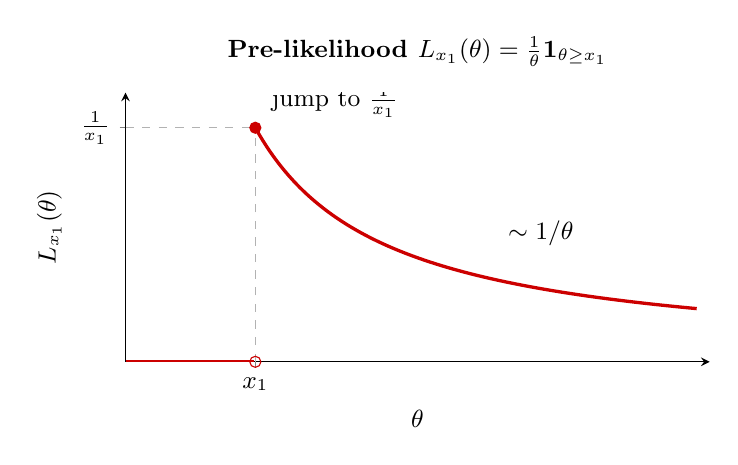
\begin{tikzpicture}
\begin{axis}[
  width=9cm, height=5cm,
  xlabel={$\theta$}, ylabel={$L_{x_1}(\theta)$},
  title={Pre-likelihood $L_{x_1}(\theta)=\tfrac{1}{\theta}\mathbf{1}_{\theta\ge x_1}$},
  xmin=0, xmax=4.5, ymin=0, ymax=1.15,
  axis lines=left,
  tick label style={font=\small},
  title style={font=\small\bfseries},
  label style={font=\small},
  xtick={1}, xticklabels={$x_1$},
  ytick={1}, yticklabels={$\tfrac{1}{x_1}$},
]
% zero for theta < x0
\addplot[very thick,red!80!black] coordinates {(0,0)(0.99,0)};
% jump discontinuity at x0=1
\addplot[very thick,red!80!black,domain=1:4.4,samples=120]{1/x};
% vertical cliff at x0
\addplot[dashed,gray!60] coordinates {(1,0)(1,1)};
\addplot[dashed,gray!60] coordinates {(0,1)(1,1)};
% open circle at theta=x0 from left
\addplot[only marks,mark=o,mark size=2pt,red!80!black]
  coordinates {(1,0)};
% filled circle at theta=x0 from right
\addplot[only marks,mark=*,mark size=2pt,red!80!black]
  coordinates {(1,1)};
\node[font=\small,anchor=south west] at (axis cs:1.05,1)
  {jump to $\tfrac{1}{x_1}$};
\node[font=\small] at (axis cs:3.2,0.55) {$\sim 1/\theta$};
\end{axis}
\end{tikzpicture}
\end{center}

The pre-likelihood is maximised at its \emph{left boundary}
$\theta = x_1$: since $1/\theta$ is decreasing, the largest value is
achieved at the smallest admissible $\theta$.  Hence the MLE from a
single observation is
\[
  \hat\theta \;=\; x_1.
\]

%--------------------------------------------------------------------
\subsection{Step 4.\ Log-pre-likelihood}
%--------------------------------------------------------------------

Taking logs on the support $\theta \ge x_1$:
\[
  \ell_{x_1}(\theta)
  \;=\; \ln h(x_1,\theta)
  \;=\; \ln\frac{1}{\theta}
  \;=\; -\ln\theta,
  \qquad \theta \ge x_1.
\]
Outside this region $\ell_{x_1}(\theta) = -\infty$ (or undefined).
The function $-\ln\theta$ is strictly \emph{decreasing}, so its
maximum is again at the left boundary $\theta = x_1$.

\begin{center}
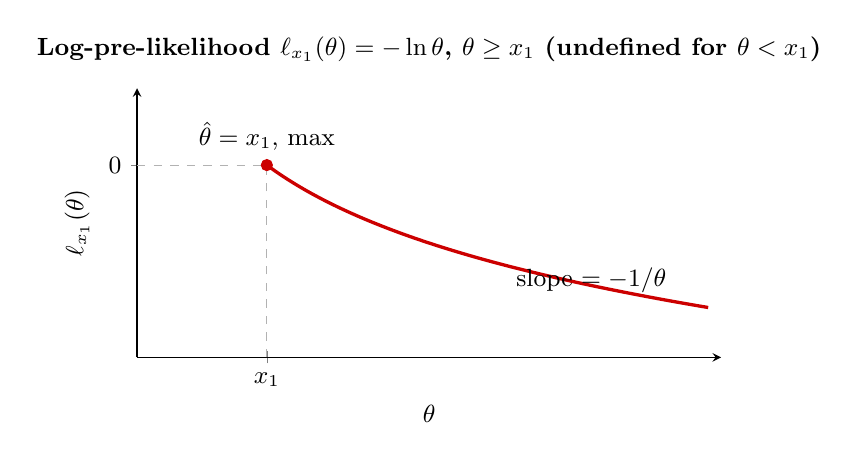
\begin{tikzpicture}
\begin{axis}[
  width=9cm, height=5cm,
  xlabel={$\theta$}, ylabel={$\ell_{x_1}(\theta)$},
  title={Log-pre-likelihood $\ell_{x_1}(\theta)=-\ln\theta$,\
    $\theta\ge x_1$ (undefined for $\theta<x_1$)},
  xmin=0, xmax=4.5, ymin=-2.0, ymax=0.8,
  axis lines=left,
  tick label style={font=\small},
  title style={font=\small\bfseries,align=center},
  label style={font=\small},
  xtick={1}, xticklabels={$x_1$},
  ytick={0}, yticklabels={$0$},
]
\addplot[very thick,red!80!black,domain=1:4.4,samples=120]{-ln(x)};
\addplot[dashed,gray!60] coordinates {(1,-2)(1,0)};
\addplot[dashed,gray!60] coordinates {(0,0)(1,0)};
\addplot[only marks,mark=*,mark size=2pt,red!80!black]
  coordinates {(1,0)};
\node[font=\small,anchor=south] at (axis cs:1,0.05)
  {$\hat\theta=x_1$, max};
\node[font=\small] at (axis cs:3.5,-1.2) {slope $=-1/\theta$};
\end{axis}
\end{tikzpicture}
\end{center}

%--------------------------------------------------------------------
\subsection{Step 5.\ $n$ observations: joint likelihood and MLE}
%--------------------------------------------------------------------

For an i.i.d.\ sample $(x_1,\ldots,x_n)$ the joint density is
\[
  h(x_1,\ldots,x_n;\theta)
  \;=\; \prod_{i=1}^n \frac{1}{\theta}\,\mathbf{1}_{x_i\le\theta}
  \;=\; \frac{1}{\theta^n}\,\mathbf{1}_{\theta\ge x_{(n)}},
\]
where $x_{(n)} = \max_i x_i$.  The constraint $\theta\ge x_i$ for all
$i$ collapses to $\theta \ge x_{(n)}$.

The joint log-likelihood is
\[
  \ell(\theta) \;=\; -n\ln\theta, \qquad \theta \ge x_{(n)}.
\]
Again a decreasing function, maximised at the left boundary:
\[
  \boxed{\hat\theta \;=\; x_{(n)} \;=\; \max(x_1,\ldots,x_n).}
\]

\begin{center}
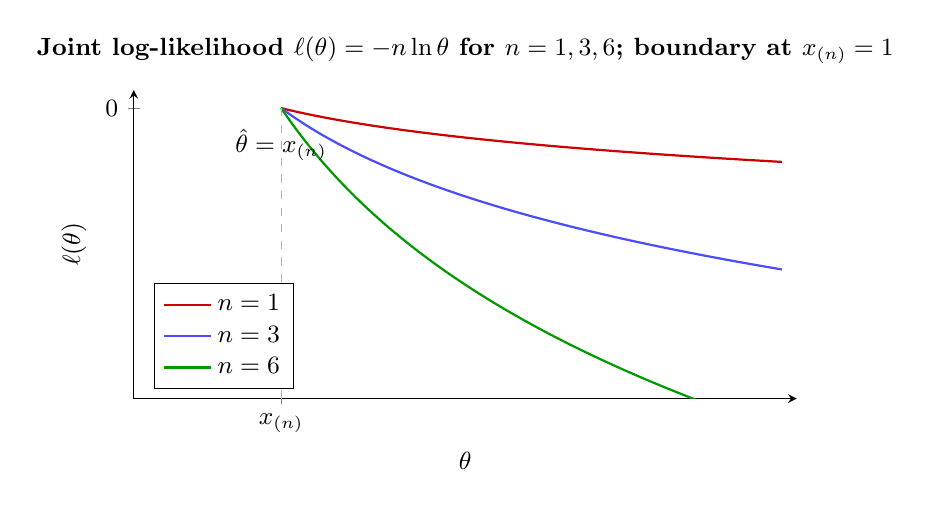
\begin{tikzpicture}
\begin{axis}[
  width=10cm, height=5.5cm,
  xlabel={$\theta$}, ylabel={$\ell(\theta)$},
  title={Joint log-likelihood $\ell(\theta)=-n\ln\theta$
    for $n=1,3,6$; boundary at $x_{(n)}=1$},
  xmin=0, xmax=4.5, ymin=-8, ymax=0.5,
  axis lines=left,
  tick label style={font=\small},
  title style={font=\small\bfseries,align=center},
  label style={font=\small},
  xtick={1}, xticklabels={$x_{(n)}$},
  ytick={0},
  legend pos=south west, legend style={font=\small},
]
\addplot[thick,red!80!black,domain=1:4.4,samples=100]{-ln(x)};
\addplot[thick,blue!70,domain=1:4.4,samples=100]{-3*ln(x)};
\addplot[thick,green!60!black,domain=1:4.4,samples=100]{-6*ln(x)};
\addplot[dashed,gray!60] coordinates {(1,-8)(1,0)};
\legend{$n=1$,$n=3$,$n=6$}
\node[font=\small,anchor=north] at (axis cs:1,-0.3)
  {$\hat\theta=x_{(n)}$};
\end{axis}
\end{tikzpicture}
\end{center}

\noindent As $n$ grows the log-likelihood steepens: each additional
observation tightens the constraint on $\theta$ from below, and the
function descends faster.


%====================================================================
\subsection{Step 5a.\ MLE: explicit derivation and consistency}
\label{sec:u0t_mle_consistency}
%====================================================================

%------------------------------------------------------------
\paragraph{$n=1$: MLE from the pre-likelihood.}

Fix $x_1 > 0$.  The pre-likelihood $L_{x_1}(\theta) =
\frac{1}{\theta}\,\mathbf{1}_{x_1 \le \theta}$ is a function of
$\theta$ with parameter $x_1$, always non-negative.

\begin{center}
\includegraphics[width=0.60\textwidth]{fig_u22_lx1_2d.png}
\end{center}

\noindent On the feasible region $\theta \ge x_1$ the function
$1/\theta$ is strictly decreasing.  Therefore the maximum is
attained at the left boundary:
\[
  \max_\theta\, L_{x_1}(\theta)
  \;=\; \frac{1}{x_1}
  \;=\; L_{x_1}(\theta)\big|_{\theta = x_1},
  \qquad
  \operatorname{argmax}_\theta\, L_{x_1}(\theta) \;=\; x_1.
\]

%------------------------------------------------------------
\paragraph{$n$ observations: sufficiency and the 3D picture.}

For $n$ i.i.d.\ observations the likelihood reduces to
$\widetilde{L}_{x_{(n)}}(\theta) = \theta^{-n}\mathbf{1}_{\theta \ge x_{(n)}}$.
The same argument applies: on $[\,x_{(n)},\infty)$ the function
$\theta^{-n}$ is strictly decreasing, so the maximum is at
$\theta = x_{(n)}$.

The Probabilist's 3D picture shows the surface $\widetilde{L}_{x_{(n)}}(\theta)$
with the cliff at $\theta = x_{(n)}$ and the MLE marked on the
$\theta$-axis:

\begin{center}
\includegraphics[width=0.72\textwidth]{fig_u22_ltilde_mle.png}
\end{center}

\begin{center}
\includegraphics[width=0.60\textwidth]{fig_u22_ltilde_top.png}
\end{center}

The full maximisation chain:
\[
  \max_\theta L_{x_1,\ldots,x_n}(\theta)
  \;=\; \max_\theta\,\widetilde{L}_{x_{(n)}}(\theta)
  \;=\; \widetilde{L}_{x_{(n)}}(\theta)\big|_{\theta=x_{(n)}},
\]
\[
  \hat\theta_{\mathrm{MLE}}(x_1,\ldots,x_n)
  \;=\; \operatorname{argmax}_\theta\, L_{x_1,\ldots,x_n}(\theta)
  \;=\; x_{(n)}(x_1,\ldots,x_n).
\]

%------------------------------------------------------------
\paragraph{Consistency: $x_{(n)} \xrightarrow{p} \theta_0$.}

\emph{Goal.} Assume $\theta = \theta_0$ is the true parameter and
$(x_1,\ldots,x_n)$ is an i.i.d.\ $\mathrm{U}[0,\theta_0]$ sample.
We want to show
\[
  X_{(n)} = \max_{i=1,\ldots,n} X_i \;\xrightarrow{p}\; \theta_0
  \quad\text{as }n\to\infty.
\]
By definition this means: for every $\varepsilon > 0$,
$P\{|X_{(n)} - \theta_0| > \varepsilon\} \to 0$.

\smallskip
\noindent\emph{Proof.} Fix $\varepsilon > 0$.  Decompose the event:
\begin{align*}
  \{|X_{(n)} - \theta_0| > \varepsilon\}
  &= \{X_{(n)} > \theta_0 + \varepsilon\} \cup \{X_{(n)} < \theta_0 - \varepsilon\}.
\end{align*}
The first event is \emph{empty} by assumption ($X_i \le \theta_0$
always, so $X_{(n)} \le \theta_0 < \theta_0 + \varepsilon$).
Therefore:
\begin{align*}
  \{|X_{(n)} - \theta_0| > \varepsilon\}
  &= \{X_{(n)} < \theta_0 - \varepsilon\}
   = \bigcap_{i=1}^n \{X_i < \theta_0 - \varepsilon\}.
\end{align*}
Taking probabilities and using independence then identical distribution:
\begin{align*}
  P\{|X_{(n)} - \theta_0| > \varepsilon\}
  &= P\!\left\{\bigcap_{i=1}^n \{X_i < \theta_0-\varepsilon\}\right\}
   \stackrel{\mathrm{ind.}}{=}
   \prod_{i=1}^n P\{X_i < \theta_0 - \varepsilon\} \\
  &\stackrel{\mathrm{i.d.}}{=}
   \Bigl(P\{X_1 < \theta_0-\varepsilon\}\Bigr)^n
   \stackrel{X\sim\mathrm{U}[0,\theta_0]}{=}
   \left(\frac{\theta_0-\varepsilon}{\theta_0}\right)^{\!n}
   \;\longrightarrow\; 0,
\end{align*}
because $\varepsilon > 0$ implies $(\theta_0-\varepsilon)/\theta_0 < 1$.\hfill$\square$

\begin{remark}[Almost sure convergence]
In fact $X_{(n)} \xrightarrow{a.s.} \theta_0$ as well, because
$X_{(n)}$ is monotone non-decreasing in $n$: adding an observation
can only increase the maximum.  A bounded monotone sequence converges
almost surely.
\end{remark}

%--------------------------------------------------------------------
\subsection{Step 6.\ Random curves}
%--------------------------------------------------------------------

Treat the data as random: $X(\omega)\sim\mathrm{U}[0,\theta_0]$.
Each $\omega$ produces one observation $X(\omega)\in[0,\theta_0]$,
and hence one pre-likelihood curve $(1/\theta)\cdot\mathbf{1}_{\theta
\ge X(\omega)}$.  Smaller observations permit smaller $\theta$
(curves start earlier); larger observations push the admissible
region to the right.  For $n=1$, since $X\sim\mathrm{U}[0,\theta_0]$,
the single observation is uniform, so the starting points of the
individual curves are indeed uniformly distributed on $[0,\theta_0]$.

\begin{center}
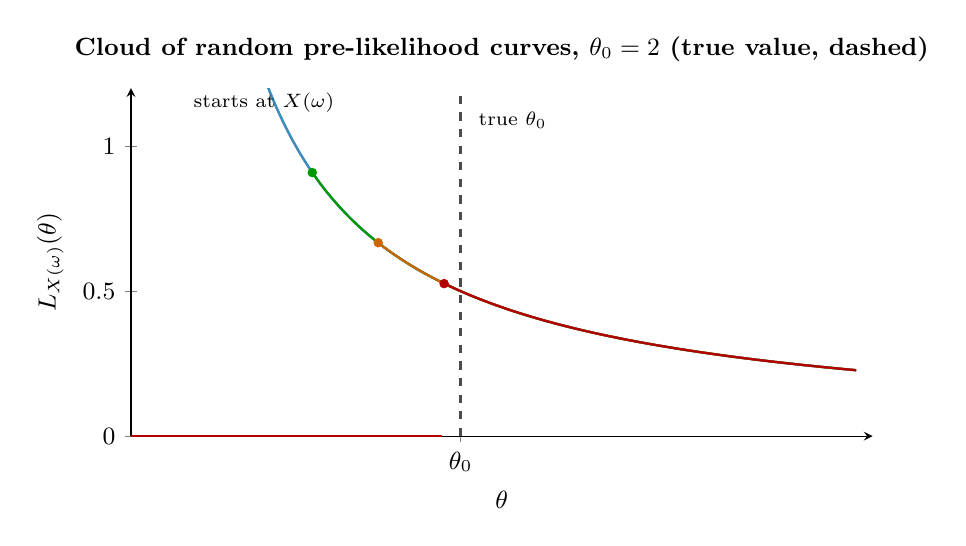
\begin{tikzpicture}[font=\small]
\begin{axis}[
  width=11cm, height=6cm,
  xlabel={$\theta$}, ylabel={$L_{X(\omega)}(\theta)$},
  title={Cloud of random pre-likelihood curves,
    $\theta_0=2$ (true value, dashed)},
  xmin=0, xmax=4.5, ymin=0, ymax=1.2,
  axis lines=left,
  tick label style={font=\small},
  title style={font=\small\bfseries,align=center},
  label style={font=\small},
  xtick={2}, xticklabels={$\theta_0$},
]
% five sample curves with x values in [0, theta0=2]
\addplot[thick,blue!60,domain=0.3:4.4,samples=80]{1/x};
\addplot[thick,blue!60] coordinates {(0,0)(0.29,0)};
\addplot[only marks,mark=*,mark size=1.5pt,blue!60] coordinates {(0.3,3.333)};

\addplot[thick,cyan!70!black,domain=0.7:4.4,samples=80]{1/x};
\addplot[thick,cyan!70!black] coordinates {(0,0)(0.69,0)};
\addplot[only marks,mark=*,mark size=1.5pt,cyan!70!black] coordinates {(0.7,1.429)};

\addplot[thick,green!60!black,domain=1.1:4.4,samples=80]{1/x};
\addplot[thick,green!60!black] coordinates {(0,0)(1.09,0)};
\addplot[only marks,mark=*,mark size=1.5pt,green!60!black] coordinates {(1.1,0.909)};

\addplot[thick,orange!80!black,domain=1.5:4.4,samples=80]{1/x};
\addplot[thick,orange!80!black] coordinates {(0,0)(1.49,0)};
\addplot[only marks,mark=*,mark size=1.5pt,orange!80!black] coordinates {(1.5,0.667)};

\addplot[thick,red!70!black,domain=1.9:4.4,samples=80]{1/x};
\addplot[thick,red!70!black] coordinates {(0,0)(1.89,0)};
\addplot[only marks,mark=*,mark size=1.5pt,red!70!black] coordinates {(1.9,0.526)};
% true theta0
\addplot[dashed,black!70,very thick] coordinates {(2,0)(2,1.2)};
\node[font=\scriptsize,anchor=north west] at (axis cs:2.05,1.15)
  {true $\theta_0$};
\node[font=\scriptsize,anchor=west] at (axis cs:0.32,1.15)
  {starts at $X(\omega)$};
\end{axis}
\end{tikzpicture}
\end{center}

\noindent All curves agree that $\theta \ge x_{\max} = \max_i
X_i(\omega)$, and each votes for the smallest possible $\theta$.
The MLE $\hat\theta = x_{(n)}$ is the smallest $\theta$ consistent
with all observed data.

\begin{remark}[Distribution of the MLE: order statistics and the Beta]
For $n > 1$ the starting point of the \emph{joint} likelihood is
$X_{(n)} = \max(X_1,\ldots,X_n)$, not a single uniform observation.
For i.i.d.\ $X_i \sim \mathrm{U}[0,\theta_0]$ the $k$-th order
statistic has the scaled Beta distribution:
\[
  X_{(k)} \;\sim\; \theta_0 \cdot \mathrm{Beta}(k,\, n-k+1),
  \qquad
  f_{X_{(k)}}(x) \;=\; \frac{n!}{(k-1)!(n-k)!}
  \left(\frac{x}{\theta_0}\right)^{k-1}
  \left(1-\frac{x}{\theta_0}\right)^{n-k}
  \frac{1}{\theta_0}.
\]
In particular the MLE $\hat\theta = X_{(n)} \sim \theta_0\cdot\mathrm{Beta}(n,1)$
has density $f(x)= n x^{n-1}/\theta_0^n$ on $[0,\theta_0]$: it is
\emph{right-skewed toward $\theta_0$}, not uniform.  Its mean and
bias are
\[
  \mathbb{E}[\hat\theta] \;=\; \frac{n}{n+1}\,\theta_0,
  \qquad
  \mathrm{Bias} \;=\; -\frac{\theta_0}{n+1} \;\to\; 0.
\]
The bias-corrected estimator $\frac{n+1}{n}\,X_{(n)}$ is unbiased.
The deviation $\theta_0 - X_{(n)}$ is $O(1/n)$ in probability,
which explains why the MLE converges at rate $1/n$ rather than
$1/\sqrt{n}$: each new observation can only shrink the gap
$[\,X_{(n)},\theta_0\,]$, and after $n$ uniform draws the expected
gap is $\theta_0/(n+1)$.

The minimum $X_{(1)} \sim \theta_0\cdot\mathrm{Beta}(1,n)$ is
left-skewed toward $0$, with mean $\theta_0/(n+1)$.  The full
picture: the $k$-th order statistic has mean
$k\theta_0/(n+1)$, so the $n$ order statistics divide
$[0,\theta_0]$ into $n+1$ equal-mean spacings --- a classical
result on uniform spacings.
\end{remark}

%====================================================================
\subsection{Step 5b.\ Multiple observations: geometry of the joint likelihood}
\label{sec:u0t_multi_geom}
%====================================================================

The joint likelihood $L_{x_1,\ldots,x_n}(\theta)$ factorises over the
i.i.d.\ sample and simplifies to a function of the order statistic
$x_{(n)} = \max_i x_i$ alone:
\[
  L_{x_1,\ldots,x_n}(\theta)
  \;=\; \prod_{i=1}^n \frac{1}{\theta}\,\mathbf{1}_{x_i \le \theta}
  \;=\; \frac{1}{\theta^n}\,\mathbf{1}_{x_{(n)}\le\theta}.
\]
The key reduction step: all $n$ constraints $x_i \le \theta$ collapse
into the single constraint $\max(x_1,\ldots,x_n) \le \theta$.

\medskip
\noindent\textbf{Number line picture.}
On the $\theta$-axis, the data $x_{(1)} \le \cdots \le x_{(n)}$
cluster to the left of $\theta$; the constraint forces $\theta$ to
the right of the largest observation.

\begin{center}
\includegraphics[width=0.65\textwidth]{fig_u21_numline.png}
\end{center}

%------------------------------------------------------------
\paragraph{The joint likelihood as a 3D surface for $n=2$.}

For $n=2$ fix $\theta$ and let $(x_1, x_2)$ vary.  The constraint
region $\{(x_1,x_2): x_1\le\theta,\, x_2\le\theta\}$ is the square
$[0,\theta]^2$; the likelihood equals $1/\theta^2$ inside and $0$
outside, forming a wedge-shaped surface above the positive quadrant.

\begin{center}
\includegraphics[width=0.70\textwidth]{fig_u21_wedge3d.png}
\end{center}

\noindent As $\theta$ increases the square grows and the height
$1/\theta^2$ decreases: more parameter space is consistent with the
data, but each point has lower density.

\medskip
\noindent\textbf{Contour view.}
The level sets of $h(x_1,x_2;\theta)$ as a function of $(x_1,x_2)$
for fixed $\theta$ are squares with the corner at the origin:
brighter (yellow) = larger $\theta$ = lower density; darker (red/purple)
= smaller $\theta$ = higher density.  The white diagonal $x_1=x_2$
marks the ridge.

\begin{center}
\includegraphics[width=0.55\textwidth]{fig_u21_contour.png}
\end{center}

%------------------------------------------------------------
\paragraph{Building $L_{x_1}(\theta)$ from two factors.}

\noindent For $n=1$ fix $x_1$ and vary $\theta$.  The pre-likelihood
$L_{x_1}(\theta)$ is the product of two bivariate functions:

\begin{enumerate}
\item The \textbf{indicator} $\mathbf{1}_{x\le\theta}$: flat value $1$
  on the region $x\le\theta$ (above the diagonal), zero below.
\item The \textbf{hyperbolic factor} $1/\theta$: a surface that depends
  only on $\theta$, declining toward the $\theta$-axis.
\end{enumerate}

\noindent\textit{Step 1: $L_{x_1}(\theta)$ for fixed $x_1$.}
The 2D section at fixed $x_1$ shows the cliff structure:
zero for $\theta < x_1$, jump to $1/x_1$ at $\theta=x_1$, then
$1/\theta$ decay.

\begin{center}
\includegraphics[width=0.60\textwidth]{fig_u21_slice2d.png}
\end{center}

\noindent\textit{Step 2: $\mathbf{1}_{x\le\theta}$ as a bivariate surface.}
Viewed as a function of both $x$ and $\theta$, the indicator is flat
($=1$) over the triangular region below the diagonal $x=\theta$, with
a vertical cliff on the ridge.  Green curtains mark the contribution
at fixed $\theta$; red hatching shows the domain constraint.

\begin{center}
\includegraphics[width=0.70\textwidth]{fig_u21_indicator3d.png}
\end{center}

\noindent\textit{Step 3: Adding the constraint $x>0$.}
The indicator $\mathbf{1}_{0 \le x \le \theta}$ restricts to
$x \ge 0$, cutting out the left half-plane.  The resulting
surface lives strictly in the first quadrant.

\begin{center}
\includegraphics[width=0.70\textwidth]{fig_u21_constraint3d.png}
\end{center}

\noindent\textit{Step 4: The factor $1/\theta$ separately.}
Viewed as a surface over the $(x,\theta)$ plane, $1/\theta$ is
a ``scroll'': flat in $x$, hyperbolic in $\theta$, declining
away from the $\theta$-axis.

\begin{center}
\includegraphics[width=0.70\textwidth]{fig_u21_theta3d.png}
\end{center}

\noindent\textit{Step 5: The product $= L_{x_1}(\theta)$ surface.}
Multiplying the constraint surface by $1/\theta$ gives the full
bivariate surface $h(x,\theta) = (1/\theta)\cdot\mathbf{1}_{0\le x\le\theta}$:
the cliff at $x=\theta$, zero for $x>\theta$, and $1/\theta$ decay
for $x<\theta$.

\begin{center}
\includegraphics[width=0.70\textwidth]{fig_u21_full3d.png}
\end{center}

%------------------------------------------------------------
\paragraph{Sufficiency: the data collapse to $x_{(n)}$.}

The key structural insight is that the $n$-dimensional data vector
$(x_1,\ldots,x_n)$ enters the likelihood \emph{only} through
$x_{(n)} = \max_i x_i$.  The Probabilist's diagram below shows the chain:
\[
  (x_1,\ldots,x_n) \;\xrightarrow{\text{max}}\; x_{(n)}
  \;\longrightarrow\; L_{x_1,\ldots,x_n}(\theta)
  \;=\; \widetilde{L}_{x_{(n)}}(\theta).
\]
This is a simple example of \textbf{sufficiency}: $x_{(n)}$
is a sufficient statistic for $\theta$ in the $\mathrm{U}[0,\theta]$
family.

\begin{center}
\includegraphics[width=0.65\textwidth]{fig_u21_sufficiency.png}
\end{center}

\noindent Once we know $x_{(n)}$, the likelihood is fully determined.
The 3D geometry collapses: the full $n$-dimensional surface reduces to
the same cliff-and-decay shape we saw for $n=1$, but now with the
cliff at $\theta = x_{(n)}$ instead of $x_1$.

\begin{center}
\includegraphics[width=0.70\textwidth]{fig_u21_reduced3d.png}
\end{center}

\begin{remark}[Homework: verify $x_{(n)}$ is MLE]
Check directly that $\hat\theta = x_{(n)}$ maximises
$L_{x_1,\ldots,x_n}(\theta) = \theta^{-n}\mathbf{1}_{\theta\ge x_{(n)}}$
over $\theta > 0$.  (Hint: the function is strictly decreasing in
$\theta$ on the feasible region $[\,x_{(n)},\infty)$.)

\medskip
\noindent\textit{Next:} check consistency of $\hat\theta = x_{(n)}$,
i.e., that $x_{(n)} \xrightarrow{p} \theta_0$ as $n\to\infty$.
\end{remark}


%--------------------------------------------------------------------

%------------------------------------------------------------------
\subsection{Step 4b.\ Log-pre-likelihood: extended treatment}
%------------------------------------------------------------------

The log-pre-likelihood for a single observation $x_1$ is
\[
  \ell_{x_1}(\theta)
  \;=\; \ln h(x_1, \theta)
  \;=\;
  \begin{cases}
    -\infty, & \theta < x_1, \\
    -\ln\theta, & \theta \ge x_1,
  \end{cases}
\]
which can be written compactly (abusing notation, $(-\infty)\cdot 0 := 0$) as
\[
  \ell_{x_1}(\theta)
  \;=\; (-\infty)\cdot\mathbf{1}_{\theta < x_1}
        \;+\; (-\ln\theta)\cdot\mathbf{1}_{\theta \ge x_1}.
\]
The MLE is therefore $\hat\theta_{\mathrm{MLE}} = \operatorname{argmax}_\theta \ell_{x_1}(\theta) = x_1$.

\medskip
\noindent The figure below shows (left) the pre-likelihood $1/\theta$
in red and (right) the log-pre-likelihood $-\ln\theta$ in blue,
for several values of $x_1 < 1$.  Each curve starts at its own $x_1$
and the log-curves all pass through the value $-\ln x_1$ at the jump.

\begin{center}
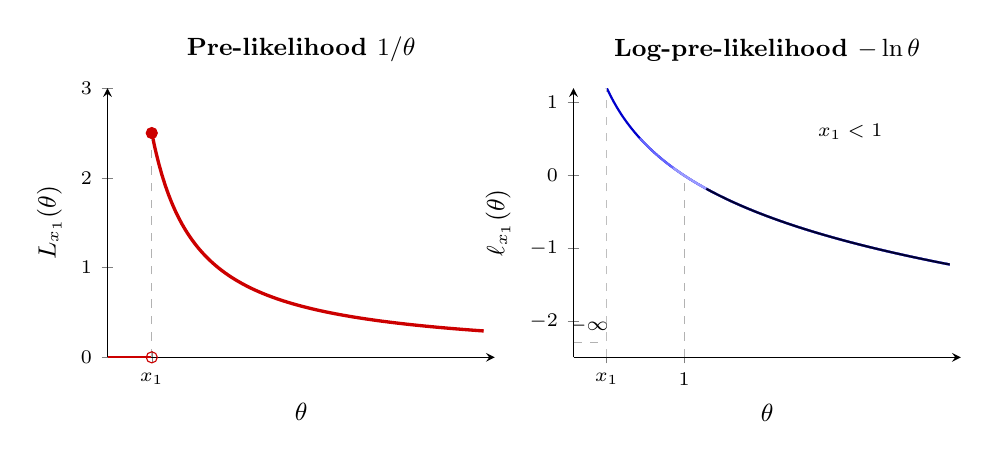
\begin{tikzpicture}
% Left panel: pre-likelihood 1/theta (red), x1=0.4
\begin{axis}[
  name=left, width=6.5cm, height=5cm,
  xlabel={$\theta$}, ylabel={$L_{x_1}(\theta)$},
  title={Pre-likelihood $1/\theta$},
  xmin=0, xmax=3.5, ymin=0, ymax=3.0,
  axis lines=left,
  tick label style={font=\scriptsize},
  title style={font=\small\bfseries},
  label style={font=\small},
  xtick={0.4}, xticklabels={$x_1$},
]
\addplot[very thick,red!80!black,domain=0.4:3.4,samples=100]{1/x};
\addplot[thick,red!80!black] coordinates{(0,0)(0.39,0)};
\addplot[only marks,mark=*,mark size=2pt,red!80!black] coordinates{(0.4,2.5)};
\addplot[only marks,mark=o,mark size=2pt,red!80!black] coordinates{(0.4,0)};
\addplot[dashed,gray!60] coordinates{(0.4,0)(0.4,2.5)};
\end{axis}
% Right panel: log-pre-likelihood -ln(theta), several x1 values (blue)
\begin{axis}[
  name=right, at={(left.east)}, anchor=west, xshift=1cm,
  width=6.5cm, height=5cm,
  xlabel={$\theta$}, ylabel={$\ell_{x_1}(\theta)$},
  title={Log-pre-likelihood $-\ln\theta$},
  xmin=0, xmax=3.5, ymin=-2.5, ymax=1.2,
  axis lines=left,
  tick label style={font=\scriptsize},
  title style={font=\small\bfseries},
  label style={font=\small},
  xtick={0.3,1}, xticklabels={$x_1$,$1$},
]
% family of curves for x1 = 0.3, 0.6, 0.9, 1.2
\addplot[thick,blue!80!black,domain=0.3:3.4,samples=100]{-ln(x)};
\addplot[only marks,mark=*,mark size=2pt,blue!80!black] coordinates{(0.3,{-ln(0.3)})};
\addplot[dashed,gray!50] coordinates{(0.3,-2.5)(0.3,{-ln(0.3)})};
\addplot[thick,blue!60,domain=0.6:3.4,samples=100]{-ln(x)};
\addplot[thick,blue!40,domain=0.9:3.4,samples=100]{-ln(x)};
\addplot[thick,blue!20!black,domain=1.2:3.4,samples=100]{-ln(x)};
% reference -inf below
\draw[dashed,gray!60] (axis cs:0,-2.3) -- (axis cs:0.28,-2.3);
\node[font=\scriptsize] at (axis cs:0.14,-2.3) [above] {$-\infty$};
\node[font=\scriptsize] at (axis cs:2.5,0.6) {$x_1<1$};
\addplot[dashed,gray!60] coordinates{(1,-2.5)(1,0)};
\end{axis}
\end{tikzpicture}
\end{center}

%------------------------------------------------------------------
\noindent\textbf{The bivariate log-likelihood surface.}
The function $\ell(x,\theta) = -\ln\theta$ (ignoring the constraint)
is a surface that depends only on $\theta$: flat in $x$, decreasing
in $\theta$.  Without the constraint it looks like a rectangular
slab tilted toward $\theta \to \infty$:

\begin{center}
\includegraphics[width=0.85\textwidth]{fig20_h_3d_noconstr.png}
\end{center}

\noindent The domain constraint $0 < x \le \theta$ cuts out the triangular
region below the diagonal $x = \theta$:

\begin{center}
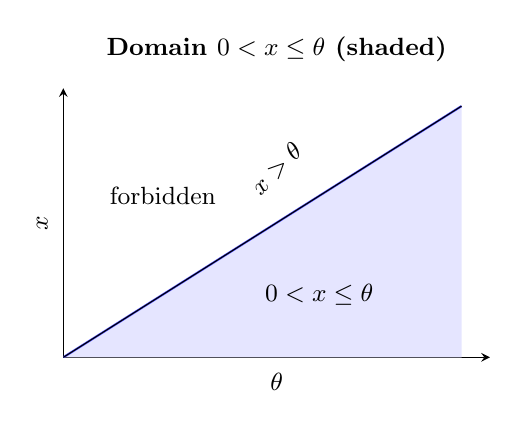
\begin{tikzpicture}
\begin{axis}[
  width=7cm, height=5cm,
  xlabel={$\theta$}, ylabel={$x$},
  title={Domain $0 < x \le \theta$ (shaded)},
  xmin=0, xmax=3, ymin=0, ymax=3,
  axis lines=left,
  tick label style={font=\small},
  title style={font=\small\bfseries},
  label style={font=\small},
  xtick=\empty, ytick=\empty,
]
% shade the region x < theta
\addplot[fill=blue!10,draw=none,domain=0:2.8,samples=2]
  {x} \closedcycle;
\addplot[thick,blue!70,domain=0:2.8,samples=2]{x};
\node[font=\small] at (axis cs:1.8,0.7) {$0<x\le\theta$};
\node[font=\small] at (axis cs:0.7,1.8) {forbidden};
% hatching the forbidden region
\addplot[pattern=north east lines,pattern color=gray!40,
  domain=0:2.8,samples=2]{x};
\node[font=\small,rotate=45] at (axis cs:1.5,2.1) {$x>\theta$};
\end{axis}
\end{tikzpicture}
\end{center}

\noindent Adding the constraint gives the full 3D log-likelihood surface
restricted to $0<x\le\theta$ (the wedge below the diagonal):

\begin{center}
\includegraphics[width=0.75\textwidth]{fig20_log_3d_constr.png}
\end{center}

\noindent Cutting this surface with the vertical plane $x = x_1$
(the $x_1$-section) extracts exactly the log-pre-likelihood $-\ln\theta$
for $\theta \ge x_1$ shown in the 2D plot above.  That section is
visible as the black curtain in the figure below:

\begin{center}
\includegraphics[width=0.80\textwidth]{fig20_log_3d_x1.png}
\end{center}

%------------------------------------------------------------------
\subsection{Step 7b.\ Pre-score: 2D and 3D geometry}
%------------------------------------------------------------------

The pre-score is the $\theta$-derivative of the log-pre-likelihood.
On the interior $\theta > x_1$ we have $\ell_{x_1}(\theta)=-\ln\theta$,
so
\[
  s_{x_1}(\theta)
  \;=\; \frac{\partial}{\partial\theta}\ell_{x_1}(\theta)
  \;=\; -\frac{1}{\theta}.
\]
For $\theta < x_1$ the log-pre-likelihood is $-\infty$ (constant), so
the derivative is zero by convention.  At $\theta = x_1$ itself there
is a jump discontinuity, so the derivative is undefined.  Formally:
\[
  s_{x_1}(\theta) \;=\;
  \begin{cases}
    0 & \text{by convention, } \theta < x_1, \\
    \text{undefined} & \theta = x_1, \\
    -1/\theta & \theta > x_1.
  \end{cases}
\]

\begin{center}
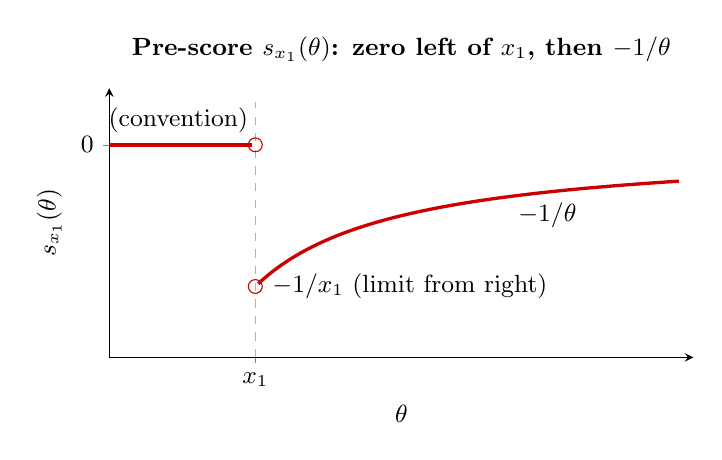
\begin{tikzpicture}
\begin{axis}[
  width=9cm, height=5cm,
  xlabel={$\theta$}, ylabel={$s_{x_1}(\theta)$},
  title={Pre-score $s_{x_1}(\theta)$: zero left of $x_1$, then $-1/\theta$},
  xmin=0, xmax=4, ymin=-1.5, ymax=0.4,
  axis lines=left,
  tick label style={font=\small},
  title style={font=\small\bfseries,align=center},
  label style={font=\small},
  xtick={1}, xticklabels={$x_1$},
  ytick={0},
]
% zero for theta < x1
\addplot[very thick,red!80!black] coordinates{(0,0)(0.98,0)};
% jump: undefined at x1=1 (open circles both sides)
\addplot[only marks,mark=o,mark size=2.5pt,red!80!black]
  coordinates{(1,0)(1,-1)};
% -1/theta for theta > x1
\addplot[very thick,red!80!black,domain=1.02:3.9,samples=100]{-1/x};
\addplot[dashed,gray!60] coordinates{(1,-1.5)(1,0.3)};
\node[font=\small,anchor=west] at (axis cs:1.05,-1.0)
  {$-1/x_1$ (limit from right)};
\node[font=\small] at (axis cs:3.0,-0.5) {$-1/\theta$};
\node[font=\small,anchor=south] at (axis cs:0.4,0.02)
  {$0$ (convention)};
\end{axis}
\end{tikzpicture}
\end{center}

\noindent Key observation: at $\theta^* = x_1$ (the MLE), the pre-score
is \emph{not} zero --- it jumps from $0$ (left) to $-1/x_1$ (right).
This is the hallmark of a non-regular family: the first-order condition
$s = 0$ fails to locate the MLE.

\medskip
\noindent\textbf{Score in 3D.}
The bivariate pre-score $s(x,\theta) = -1/\theta$ (ignoring the
constraint) is a surface that depends only on $\theta$: flat in $x$,
negative for all $\theta > 0$, increasing toward zero as
$\theta \to \infty$.  Without the constraint it is a flat red slab
below the $(x,\theta)$-plane:

\begin{center}
\includegraphics[width=0.80\textwidth]{fig20_score_3d_noconstr.png}
\end{center}

\noindent The constraint $0 < x < \theta$ is slightly more restrictive
for the score than for the log-likelihood: the diagonal $x = \theta$
itself is \emph{forbidden} (the density is zero there, so the score
is undefined on the boundary), not merely a cliff edge.  The domain
$0 < x < \theta$ (strict inequalities) is the open triangular wedge:

\begin{center}
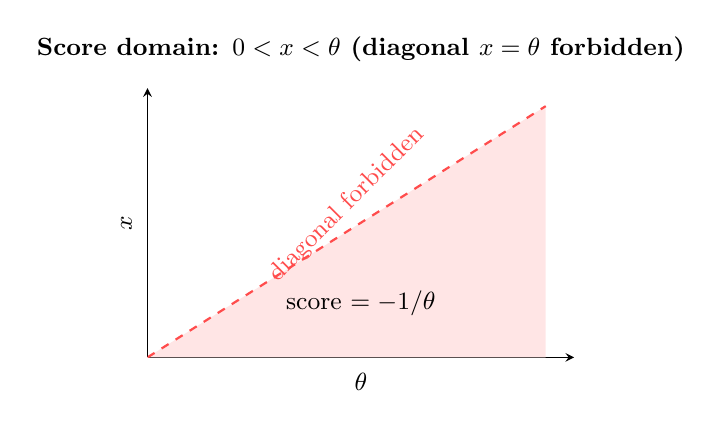
\begin{tikzpicture}
\begin{axis}[
  width=7cm, height=5cm,
  xlabel={$\theta$}, ylabel={$x$},
  title={Score domain: $0<x<\theta$ (diagonal $x=\theta$ forbidden)},
  xmin=0, xmax=3, ymin=0, ymax=3,
  axis lines=left,
  tick label style={font=\small},
  title style={font=\small\bfseries,align=center},
  label style={font=\small},
  xtick=\empty, ytick=\empty,
]
\addplot[fill=red!10,draw=none,domain=0:2.8,samples=2]
  {x} \closedcycle;
\addplot[dashed,red!70,thick,domain=0:2.8,samples=2]{x};
\node[font=\small] at (axis cs:1.5,0.6) {score $=-1/\theta$};
\node[font=\small,rotate=45,text=red!70] at (axis cs:1.4,1.7)
  {diagonal forbidden};
\end{axis}
\end{tikzpicture}
\end{center}

\noindent Adding the constraint (but before cutting with $x_1$) and
then adding the $x_1$-section gives the full picture:

\begin{center}
\includegraphics[width=0.80\textwidth]{fig20_score_3d_x1.png}
\end{center}

\noindent The $x_1$-section (blue curtain) shows the pre-score
$s_{x_1}(\theta)$: zero for $\theta < x_1$, then jumping to $-1/x_1$
and decreasing as $-1/\theta$ for $\theta > x_1$.

%------------------------------------------------------------------
\subsection{Step 8.\ Score for $n$ observations}
%------------------------------------------------------------------

%------------------------------------------------------------------
\paragraph{Recall: pre-score for $n=1$.}

For a single observation the pre-score $s_{x_1}(\theta)$ is zero
(by convention) left of $x_1$, undefined at $x_1$, and $-1/\theta$
to the right:
\[
  s_{x_1}(\theta) \;=\;
  \begin{cases}
    0 & \theta < x_1, \\
    \text{undefined} & \theta = x_1, \\
    -1/\theta & \theta > x_1.
  \end{cases}
\]

\begin{center}
\includegraphics[width=0.55\textwidth]{score_fig1.png}
\end{center}

%------------------------------------------------------------------
\paragraph{How to logarithm an indicator.}

A key step in passing from the likelihood to the log-likelihood for
$n$ observations is handling $\ln\mathbf{1}_A(\theta)$.  The
indicator $\mathbf{1}_A$ is 1 on $A$ and 0 off $A$; its logarithm
is 0 on $A$ and $-\infty$ off $A$:
\[
  \ln\mathbf{1}_A(\theta) \;=\;
  \begin{cases} 0 & \theta\in A,\\ -\infty & \theta\notin A. \end{cases}
\]

\begin{center}
\includegraphics[width=0.55\textwidth]{score_fig2.png}
\end{center}

\begin{center}
\includegraphics[width=0.60\textwidth]{score_fig3.png}
\end{center}

\noindent The product $\prod_i \frac{1}{\theta}\mathbf{1}_{x_i\le\theta}$
collapses under the log to
\[
  \ell_{x_1,\ldots,x_n}(\theta)
  \;=\; \ln\frac{1}{\theta^n} + \ln\mathbf{1}_{x_{(n)}\le\theta}
  \;=\; -n\ln\theta + 0
  \;=\; -n\ln\theta, \qquad \theta \ge x_{(n)}.
\]

%------------------------------------------------------------------
\paragraph{Score for $n$ observations.}

Differentiating gives:
\[
  s(\mathbf{x},\theta)
  \;=\;
  \begin{cases}
    -n/\theta & \theta > x_{(n)}, \\
    \text{undefined} & \theta = x_{(n)}, \\
    0 \text{ (by convention)} & \theta < x_{(n)}.
  \end{cases}
\]
Note that where the score is defined, it equals the sum of the
individual pre-scores:
$s_{x_1,\ldots,x_n}(\theta) = s_{x_1}(\theta) + \cdots + s_{x_n}(\theta)$,
valid on their common domain $\theta > x_{(n)}$.

\medskip
The 2D graph of $s$ as a function of $\theta$ (analogous to the
$n=1$ picture above, but with $x_{(n)}$ as the cliff and $-n/\theta$
on the right):

\begin{center}
\includegraphics[width=0.60\textwidth]{score_fig_n.png}
\end{center}

%------------------------------------------------------------------
\paragraph{Support, kernel, and where the cliff lives.}

Viewed as a function of $\theta$ alone, the score has two regions:
\begin{itemize}
\item \textbf{Support region} $\theta > x_{(n)}$: score $= -n/\theta$.
  It does not depend on $\mathbf{x}$ at all --- only on $\theta$.
\item \textbf{Kernel region} $\theta < x_{(n)}$: score $= 0$ by
  convention.  It also does not depend on the sample --- it is
  identically zero regardless of which $\mathbf{x}$ was observed.
\end{itemize}
In both regions the score is constant as a function of $\mathbf{x}$.
Yet the two regions are not the same: \emph{the boundary between them
--- the cliff --- depends on the sample through $x_{(n)} = \max_i
x_i$}.  The data determines where the jump is, not what the score
value is on either side of it.

%------------------------------------------------------------------
\paragraph{Score as a map: setting up the expectation.}

To compute $\E_\theta[s(\mathbf{X},\theta)]$ we have to be precise
about what ``expectation'' means here.  The score is a \emph{map}:
\[
  s(\,\cdot\,,\theta)\colon \mathbf{x} \;\longmapsto\; s(\mathbf{x},\theta).
\]
Taking its expectation means: generate the sample $\mathbf{X}$ from
the same $\theta$ that appears in the score formula, then push the
measure forward through this map.  The map and the measure it acts on
must be in agreement --- we use one and the same $\theta$ for both.

Under $\mathrm{U}[0,\theta]$, each $X_i$ lies in the open interval
$(0,\theta)$ with probability one.  Therefore $x_{(n)} < \theta$
almost surely, and the realised sample falls in the support region
with probability one:
\[
  X_i \in (0,\theta) \;\text{ a.s.}
\]

%------------------------------------------------------------------
\paragraph{Not centered, and drifting farther from zero with $n$.}

In the support region the score equals $-n/\theta$ --- constant in
$\mathbf{x}$, and still less dependent on $\omega$.  The expectation
is therefore
\[
  \E_\theta\bigl[s(\mathbf{X},\theta)\bigr]
  \;=\; \int_{[0,\theta]^n}
        \!\!\left(-\frac{n}{\theta}\right) \frac{1}{\theta^n}\,d\mathbf{x}
  \;=\; -\frac{n}{\theta}.
\]
The score identity $\E[s]=0$ fails completely, and the magnitude
$n/\theta$ grows without bound as $n\to\infty$.  Far from converging
to zero, the expected score drifts farther from it with every
additional observation.

The value $0$ in the kernel region is a \emph{conventional}
assignment --- the derivative of the constant $-\infty$ --- not a
value that the score actually takes when the sample is generated from
$\theta$.  Zero is never the true computed score; it only
appears as a bookkeeping convention at the boundary and beyond.

Finally, the score at the MLE is \emph{undefined}: $\hat\theta =
x_{(n)}$ is exactly the cliff point where the log-likelihood has a
jump discontinuity and the derivative does not exist.  The first-order
condition $s = 0$, which locates the MLE in regular families, has no
counterpart here.

\subsection{Step 7.\ Score and the failure of regularity}
%--------------------------------------------------------------------

On the interior of the support $x\in(0,\theta)$, where $h>0$, the
pre-score is
\[
  s(x,\theta)
  \;=\; \frac{\partial}{\partial\theta}\ln h(x,\theta)
  \;=\; \frac{\partial}{\partial\theta}\ln\frac{1}{\theta}
  \;=\; \frac{\partial}{\partial\theta}(-\ln\theta)
  \;=\; -\frac{1}{\theta}.
\]

\begin{center}
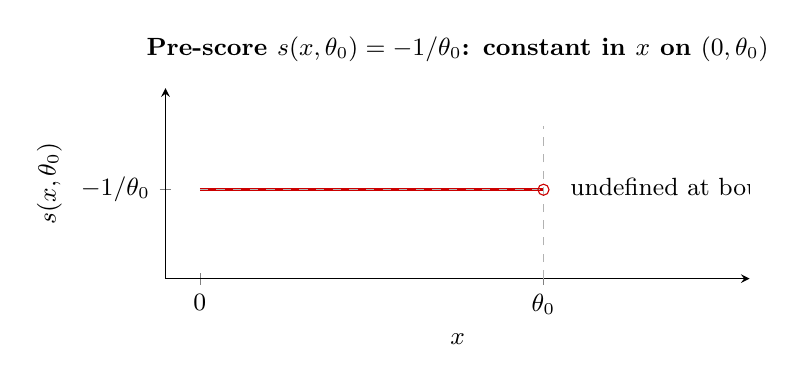
\begin{tikzpicture}
\begin{axis}[
  width=9cm, height=4cm,
  xlabel={$x$}, ylabel={$s(x,\theta_0)$},
  title={Pre-score $s(x,\theta_0)=-1/\theta_0$: constant in $x$ on $(0,\theta_0)$},
  xmin=-0.2, xmax=3.2, ymin=-1.2, ymax=0.3,
  axis lines=left,
  tick label style={font=\small},
  title style={font=\small\bfseries,align=center},
  label style={font=\small},
  xtick={0,2}, xticklabels={$0$,$\theta_0$},
  ytick={-0.5}, yticklabels={$-1/\theta_0$},
]
\addplot[very thick,red!80!black] coordinates {(0,-0.5)(2,-0.5)};
\addplot[dashed,gray!60] coordinates {(2,-1.2)(2,0)};
\addplot[dashed,gray!60] coordinates {(0,-0.5)(2,-0.5)};
\addplot[only marks,mark=o,mark size=2pt,red!80!black]
  coordinates {(2,-0.5)};
\node[font=\small,anchor=west] at (axis cs:2.1,-0.5)
  {undefined at boundary};
\end{axis}
\end{tikzpicture}
\end{center}

\medskip
\noindent\textbf{Three things go wrong simultaneously.}

\begin{itemize}
\item \textbf{Score identity fails.}
  The score $s(x,\theta) = -1/\theta$ does not depend on $x$ at all.
  Its expectation under $\mathrm{U}[0,\theta]$ is
  \[
    \E_\theta[s(X,\theta)]
    \;=\; \int_0^\theta \!\!\left(-\frac{1}{\theta}\right)
    \frac{1}{\theta}\,dx
    \;=\; -\frac{1}{\theta} \;\neq\; 0.
  \]
  The score identity $\E[s]=0$ fails because the support boundary
  $x=\theta$ depends on $\theta$; differentiating under the integral
  sign (Leibniz rule) is not valid here.

\item \textbf{Score is degenerate.}
  Since $s(x,\theta)=-1/\theta$ is constant in $x$, it is not a
  random variable in any useful sense: it carries no information
  about the specific realisation.  Its variance is zero, so the
  Fisher information $\mathcal{I}(\theta)=\Var_\theta[s]=0$ by the
  usual formula.  (The true information is finite but must be computed
  differently for non-regular families.)

\item \textbf{MLE is not found by score $= 0$.}
  The log-likelihood $\ell(\theta)=-n\ln\theta$ has derivative
  $-n/\theta\ne 0$ everywhere on its support $[\,x_{(n)},\infty)$.
  The maximum is at the \emph{left boundary} $\hat\theta=x_{(n)}$,
  not at an interior critical point.  Score-based first-order
  conditions are inapplicable.
\end{itemize}

\paragraph{CLT for score does not apply.}
In the normal example, the standardised score
$S_n/\sqrt{n\mathcal{I}(\theta_0)}\xrightarrow{d}\mathcal{N}(0,1)$
because the score is centred ($\E[s]=0$) and has finite variance.
For $\mathrm{U}[0,\theta]$ neither condition holds.  The sample
maximum $x_{(n)}$ converges to $\theta_0$ at rate $n$ (not $\sqrt{n}$,
not $\log n$): one verifies directly that for $z\ge 0$
\[
  P\bigl(n(\theta_0 - X_{(n)}) > z\bigr)
  \;=\; \Bigl(1 - \tfrac{z}{n\theta_0}\Bigr)^n
  \;\longrightarrow\; e^{-z/\theta_0},
\]
so $n(\theta_0 - X_{(n)})\xrightarrow{d}\mathrm{Exp}(1/\theta_0)$ ---
an Exponential distribution (the reversed Weibull extreme-value
distribution with shape parameter 1).  Compare: for
$X_i\sim\mathrm{Exp}(\lambda)$ the normalising sequence for the
maximum is $\log n$, not $n$, because that distribution has no
finite right endpoint.  The score-based Rao (Lagrange multiplier)
test has no counterpart in this family.

\paragraph{Summary.}
\begin{center}
\renewcommand{\arraystretch}{1.35}
\begin{tabular}{lll}
\hline
& $\mathcal{N}(\mu,1)$ & $\mathrm{U}[0,\theta]$ \\
\hline
MLE & $\bar x$ (score $=0$) & $x_{(n)}$ (boundary) \\
Score $s$  & $x-\mu$, random in $x$ & $-1/\theta$, constant in $x$ \\
$\E[s]$    & $0$ (regular)          & $-1/\theta\ne 0$ (non-regular) \\
$\Var[s]$  & $1$ (Fisher info)      & $0$ (degenerate) \\
Rate of $\hat\theta$ & $1/\sqrt{n}$ & $1/n$ \\
CLT for score & Yes (Wald, LR, Rao) & No \\
\hline
\end{tabular}
\end{center}

%--------------------------------------------------------------------
\end{document}
